\documentclass[11pt]{article}
\usepackage{fancyhdr}
\usepackage[letterpaper, margin=1in]{geometry}
%\usepackage{indentfirst}
\usepackage{graphicx}
\usepackage{amsmath}
\usepackage{amssymb}
\usepackage{siunitx}
\sisetup{detect-weight=true, detect-family=true} % makes siunitx follow font formatting like bold, italic, etc.
\usepackage{cancel}
\usepackage{isotope}
\usepackage{listings}
\usepackage[dvipsnames,table]{xcolor}
\usepackage{xspace}
\usepackage{booktabs} % makes tables pretty
\usepackage{longtable} % for long tables
\usepackage{multirow} % makes tables pretty
\usepackage{multicol} % makes tables pretty
\usepackage{setspace}
\usepackage[font={bf}]{caption}
\usepackage{subcaption}
\usepackage{hyperref}
\usepackage{cleveref}
\newcommand{\creflastconjunction}{, and\nobreakspace} % adds oxford comma to cleveref
\usepackage[utf8]{inputenc}
\usepackage{textcomp}
\usepackage{titlesec}
\usepackage{svg}
\usepackage{pdflscape} % makes pages landscape
\usepackage{mathtools}
\usepackage{enumitem}
\usepackage[T1]{fontenc}
\usepackage{tikz}

\doublespacing

% bib if needed
\bibliographystyle{ieeetr}


% fancy header stuff
\usepackage{fancyhdr}
\pagestyle{fancy}

\setlength{\headheight}{28pt}
\lhead{NSE 667\\Spring 2022}
\chead{Critical Flow\\}
\rhead{Austin Warren\\Due June 3, 2022}

\begin{document}
Calculate the critical mass flows and the corresponding back pressures if the tank is filled with saturated liquid at a pressure of 35 bar, using HEM, Fauske, and Moody models. The general assumptions are listed below.
\begin{itemize}
    \item Adiabatic process without friction loss (isentropic)
    \item Thermodynamics equilibrium quality $x_{th}$ equals the flow quality $x$
    \item Steady-state
\end{itemize}
% 
The general approach is to use the following expression that relates mass flux with enthalpy.
\begin{equation}
    G_m = \rho_m \sqrt{2 \left( h_{m,0} - h_m \right)}\:,
\end{equation}
where
\begin{equation}
    \rho_m = \left( \frac{x_{th}}{\rho_g} + \frac{1-x_{th}}{\rho_f} \right)^{-1}\:.
\end{equation}
Each model has its own modified expression, which will be listed in each section. The enthalpy can be used to determine the exit pressure. Since the process is assumed to be isentropic, we can determine the entropy of each phase at the exit.
\begin{equation}
    S_0 = S_e = S_v x + \left( 1-x \right) S_f
\end{equation}
I generated a list of exit pressure values ranging from zero to the initial pressure condition, used the exit pressure and the exit entropy to determine the exit enthalpies, densities, and quality, then used those values to determine the mass flux. All properties were determined using steam tables provided in the \textit{pyXSteam} package \cite{pyXSteam,XSteam,IAPWS97}.

The initial conditions determined from the given saturated liquid pressure are listed in \Cref{tab:init}.

\begin{table}[htbp]
    \centering
    \caption{Initial conditions}
    \begin{tabular}{cc}
        \toprule
        Parameter & Value\\
        \midrule
        $P$ & \SI{35}{bar}\\
        $T$ & \SI{242.56}{\celsius}\\
        $h_f$ & \SI{1049.78}{\kilo\joule\per\kilo\gram}\\
        $s_f$ & \SI{2.73}{\kilo\joule\per\kilo\gram\per\kelvin}\\
        \bottomrule
    \end{tabular}
    \label{tab:init}
\end{table}

\begin{enumerate}
    \item HEM Model:
    \begin{equation}
        G_m = \rho_m \sqrt{2 \left( h_{m,0} - h_m \right)}
    \end{equation}
    
    
    
    %\clearpage
    %
    \item Fauske Model:
    For models with slip:
    \begin{equation}
        G_m = \frac{\sqrt{2 \left( h_{m,0} - h_m \right)}}{\left[ \frac{x}{\rho_g} + \frac{\left( 1-x \right)}{\rho_f} S \right] \left[ x + \left( 1-x \right)\frac{1}{S^2} \right]^{1/2}}\:.
    \end{equation}
    The Fauske model:
    \begin{equation}
        S = \left( \frac{\rho_f}{\rho_g} \right)^{1/2}\:,
    \end{equation}
    \begin{equation}
        G_m = \frac{\sqrt{2 \left( h_{m,0} - h_m \right)}}{\left[ \frac{x}{\rho_g^{1/2}} + \frac{\left( 1-x \right)}{\rho_f^{1/2}} \right] \left[ \frac{x}{\rho_g} + \frac{\left( 1-x \right)}{\rho_f} \right]^{1/2}}\:.
    \end{equation}
    
    
    
    %\clearpage
    %
    \item Moody Model:
    \begin{equation}
        S = \left( \frac{\rho_f}{\rho_g} \right)^{1/3}
    \end{equation}
    



\end{enumerate}
Results are displayed on the following pages.

\clearpage
\Cref{fig:mass flow} shows the mass flux and corresponding exit pressures for all three models. It looks very similar to the example provided, with HEM having the lowest critical flow, and the Moody model having the greatest.
\begin{figure}[htbp]
    \centering
    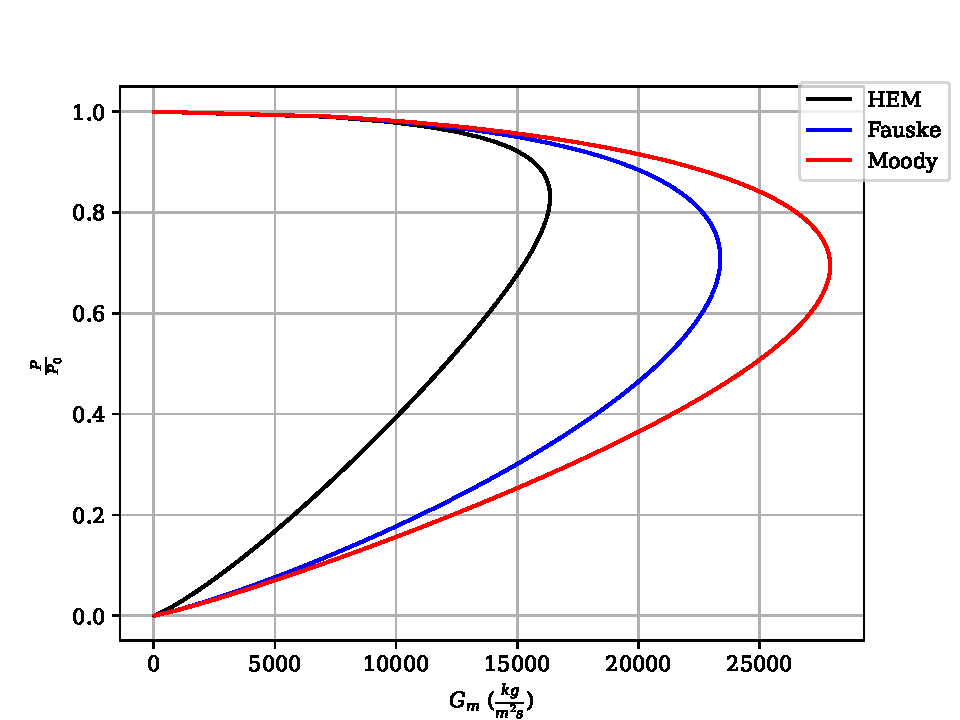
\includegraphics[width=\textwidth]{1-plots/graph_Gm.pdf}
    \caption{Mass flux vs normalized exit pressure for HEM, Fauske, and Moody models.}
    \label{fig:mass flow}
\end{figure}

\Cref{tab:crit} lists the critical values of pressure and mass flux for all three models. The maximum listed values match up well with what the plot shows. The HEM model produces the lowest mass flux value and the Moody model produces the largest. It is also interesting to note that the critical point occurs at a larger exit pressure for HEM than for the other models. (Sorry for the formatting in this table, python was not cooperating.)
\begin{table}[htbp]
	 \centering
	 \caption{Critical mass flow and back pressure.}
	 \begin{tabular}{cccc}
		 \toprule
		  & HEM & Fauske & Moody \\ 
		 \midrule 
		 $G_m \left(\si{\kilo\gram\per\meter^2\per\second}\right)$  & 16356.815282407637 & 23384.90741250147 &  27917.42946073328\\ 
		 $P_{crit}$ (bar) & 29.075600560056007 & 24.79939493949395 &  24.298987898789882 \\ 
		 \bottomrule 
	 \end{tabular} 
	 \label{tab:crit} 
\end{table}





\clearpage
% bib / works cited
\bibliography{bibliography.bib}

\end{document}
